\documentclass[12pt,a4paper]{article}



%%%%% PREAMBLE
\usepackage[margin=1in]{geometry}
%% You can use this to adjust the top bottom, left and right margins individually
\usepackage{xcolor} %gives color
\usepackage{amsmath,amssymb}
\usepackage{graphicx} %graphics package
\usepackage{subcaption} %subfigure
\usepackage{float}
\usepackage{natbib} %bibliography
\usepackage{authblk}


%%%%%%%%%%% Title page
\title{Beryllium!!!!!}
    \author{Veda}
    \affil{University of California Los Angeles}
    \date{}


%%%%%%%%%%%% Document starts here    
\begin{document}
    \maketitle
%% Section starts here
    \section{Toxicity}
    Here we talk about toxicity of Beryllium
    \subsection{The reason} %creates a subsection
    I do not know the reason

    \subsubsection{The sub-reason} %creates a subsubsection
    I do not know the sub-reason as well


    %Creating sections without numbering
     \section*{A. Alphabet Toxicity}


%%%% Section
\section{Font formatting}
Here we look at font color and style
\subsection{Font Color}
\textcolor{purple}{Is this purple?- Yes it is!!!}
\subsection{Font Style}
\textbf{This text should be bold}\\ %new line
\textit{This one is italic}
%space creates new paragraph

\textbf{\textit{This one is both!}}

\noindent \textbf{\textit{This one is both!}}

\section{Equations}
Let's learn to type various styles of equations
%%%% Make a list
\begin{itemize}
    \item The equation for straight line is 
    \begin{equation}
        y=mx+b
        \label{eq:straight_line}
    \end{equation}
    \item Inline equation: $y=mx+b$
    \item Non-numbered equation
    \begin{equation*}
        y=mx+b
    \end{equation*}
    \item Now I want to refer to equation 1. I like straightlines as shown in Eq.~\ref{eq:straight_line}.

    \item Lets do complicated equation
    \begin{equation}
        f(x)=\frac{1}{2\pi}\int_{-\infty}^{\infty} e^{-ix\xi}\left(1+\frac{\sin(\xi)}{\xi}\right) d\xi^2
    \end{equation}

    \item Alright lots of equations
    \begin{align}
        x^2+\left(\frac{5}{4} y-\sqrt{|x|} \right)^2 &= 1\\ %heart
        x^2+y^2 &= 1 %circle
    \end{align}

    \item Partial derivation : mass conservation
    \begin{equation}
        \frac{\partial \rho}{\partial t }+\frac{\partial \rho u}{\partial x}=0
    \end{equation}
    
    
\end{itemize}

\section{Adding figures}
% Holding floating figures
\begin{figure} %replace h with 't', 'b'
    \centering
    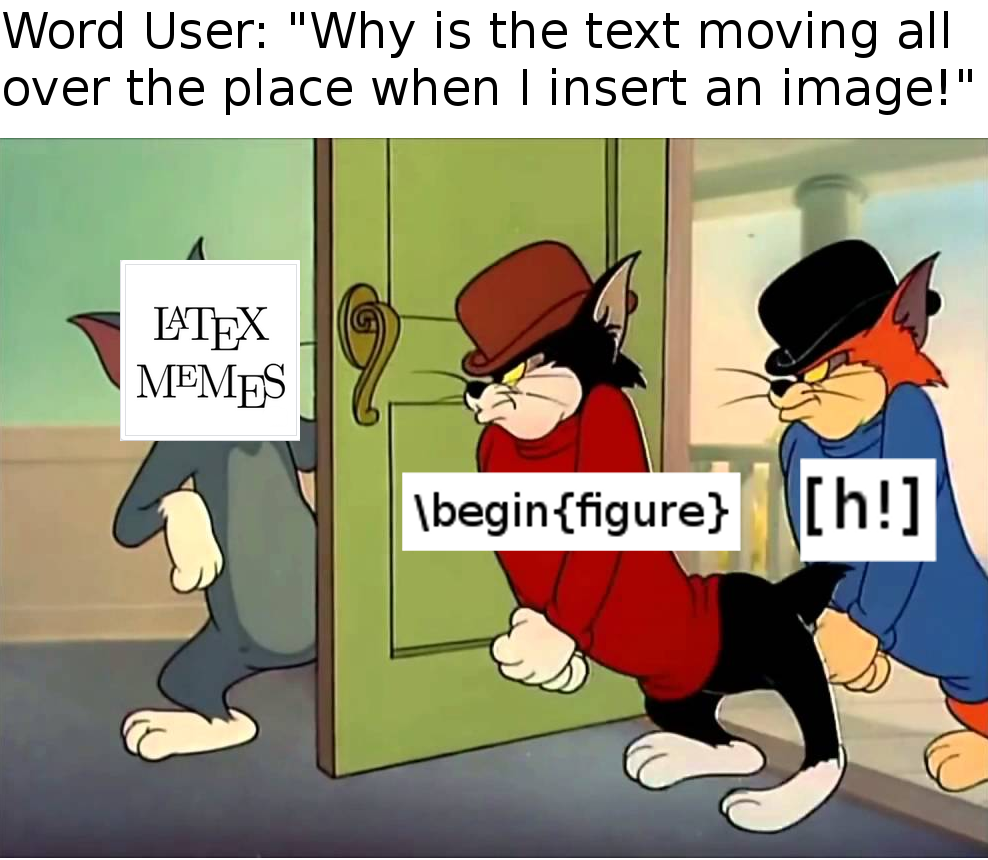
\includegraphics[width=0.5\textwidth]{figures/beginfigurememe.png}
    \caption{Meme}
    \label{fig:meme_figure}
\end{figure}

\subsection{Subfigures}
%\vspace{-10em}
\begin{figure}

    \begin{subfigure}[t]{0.4\textwidth}
    \centering
    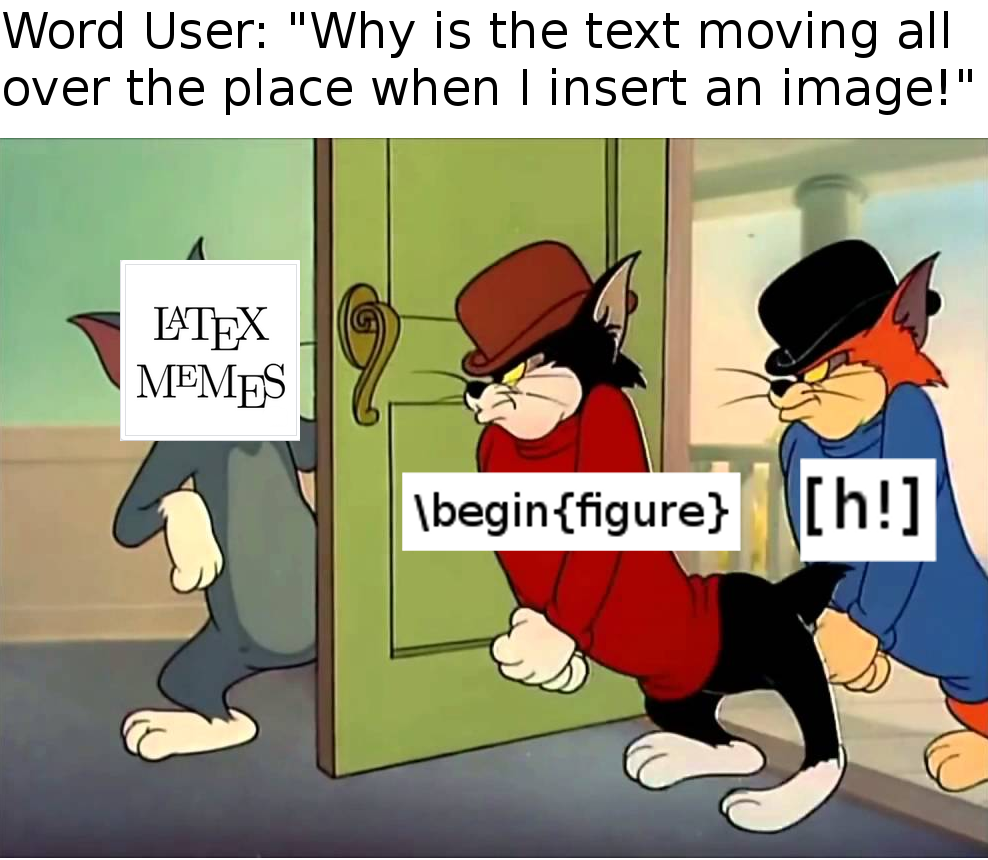
\includegraphics[width=0.5\textwidth]{figures/beginfigurememe.png}
    \caption{Tiny meme}
    \end{subfigure}
   \hspace{1em} %horizontal space
    \begin{subfigure}[t]{0.4\textwidth}
    \centering
    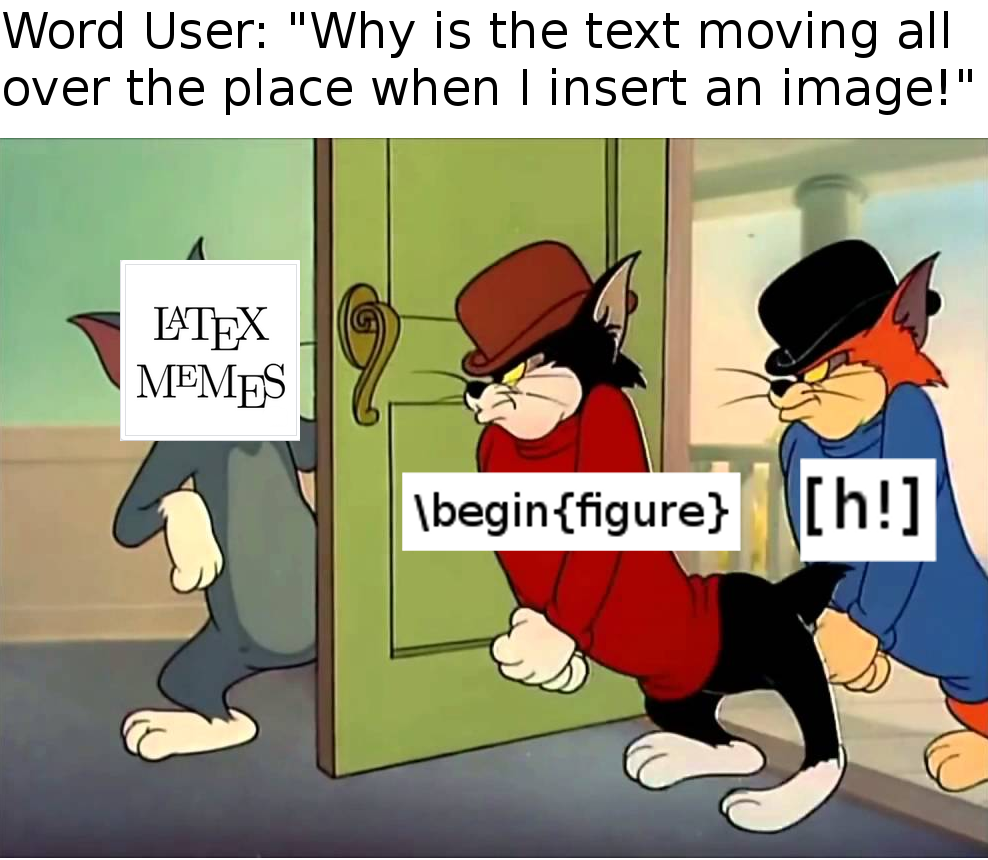
\includegraphics[width=\textwidth]{figures/beginfigurememe.png}
    \caption{Bigger meme}
    \end{subfigure}
    \caption{Duplicate memes}
    \label{fig:meme_subfigure}
\end{figure}


\section{References}
Figures could also to be taken from \cite{yuan2021wave}.

\bibliographystyle{plain} %default
\bibliography{sources}
    
\end{document}
\end{document}